%=================AVANCES Y PRUEBAS=================
% SENSORES DE PULSO

\section{API REST}
Actualmente las API REST permiten poder enviar y recibir datos de forma sencilla y rápida, es por eso que para el presente trabajo terminal y desarrollo de In-Help se utilizo un API para el envio y consulta de datos. Con ayuda de HTTP y los métodos que este permite implementar es como se comunica la Aplicación móvil (Android) con nuestra base de datos (MySQL).\\


Una de las razones por la cual se utiliza el API es que nos proporciona comunicación de manera especifica con nuestra aplicación y permite separar nuestro cliente, en este caso la aplicación den Android, de nuestro servidor, esto con un lenguaje de intercambio JSON.

\subsection{Métodos}
Para el correcto y eficiente fncionamiento en el desarrollo de la aplicación, es necesario utilizar diferentes tipos de peticiones, las cuales nos servirán para tener una omunicación entre el cliente y el servidor. Algunas de las peticiones utilizados se muestran en la figura 
\begin{figure}[htbp!]
	\centering
	\fbox{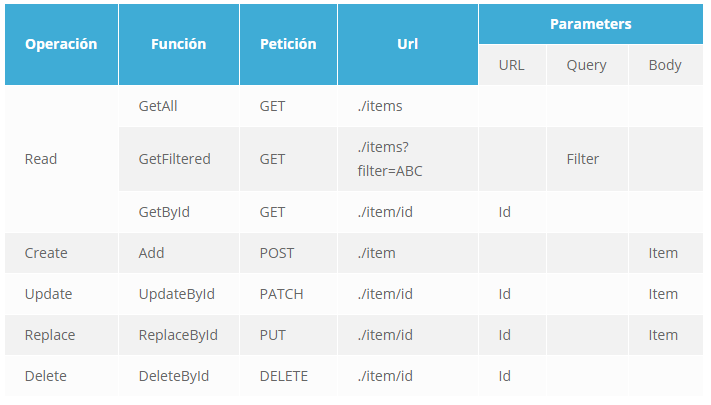
\includegraphics[width=0.9\textwidth]{AvancesPruebas/imagenes/Peticiones}}
	\caption{Peticiones}
	\label{fig:API_Peticion}
\end{figure}

 \subsection{Express}
 El index necesario para poder crear un API con Node JS y Express se muestra en la figura \ref{fig:Index}, aqui es donde se declaran los archivos de las diferentes rutas que se utilizarán, así como la inicialñización del servidor con express. En este caso debemos definir un puerto, por medio del cual el API podrá escuchar, en este caso tenemos el puerto 3000.
 
 \begin{figure}[htbp!]
 	\centering
 	\fbox{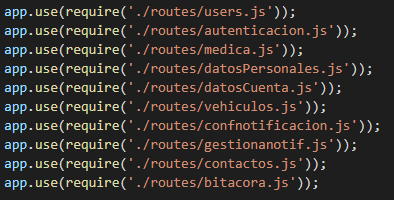
\includegraphics[width=0.9\textwidth]{AvancesPruebas/imagenes/Rutas}}
 	\caption{Index}
 	\label{fig:Index}
 \end{figure}
 \subsection{Rutas}
 
 Para que se pueda manejar de una mejor manera las peticiones que utilizamos para el funcionamiento de la aplicación, se diseño un archivo de rutas para cada uno de los diferentes módulos de la aplicación, las cuales se muestran en la figura \ref{fig:Rutas}.

\begin{figure}[htbp!]
	\centering
	\fbox{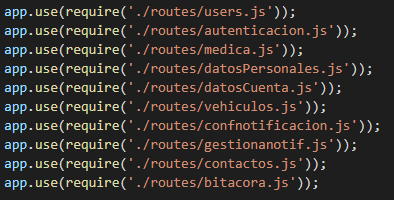
\includegraphics[width=0.9\textwidth]{AvancesPruebas/imagenes/Rutas}}
	\caption{Rutas}
	\label{fig:Rutas}
\end{figure}

 \subsection{Conexión}
 
 Para poder hacer uso de la información de nuestra base de datos se debe tener conexión a la misma desde nuestra API, es por eso que se debe crear una conexión como se muestra en la figura \ref{fig:Conexion}, donde host es el lugar donde se encuentra alojada nuestra base , y database es el nombre de nuestra base de datos.
 
 \begin{figure}[htbp!]
 	\centering
 	\fbox{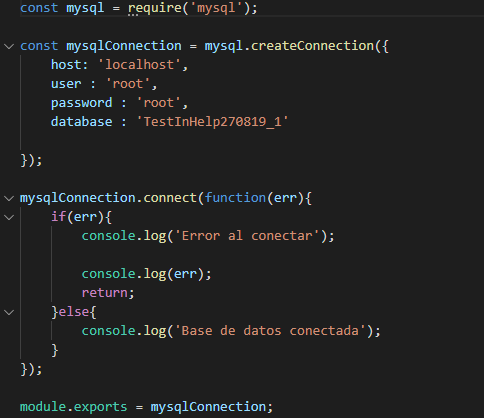
\includegraphics[width=0.9\textwidth]{AvancesPruebas/imagenes/Conexion}}
 	\caption{Conexión}
 	\label{fig:Conexion}
 \end{figure}